\chapter{Adresses MAC et probes requests}
\label{ch:probe_req}

Afin de pouvoir détecter et tracer les différents périphériques réseau présents
pendant les scans, il est impératif de pouvoir les identifier de manière unique et irrévocable.

Pour cela, nous allons utiliser l'adresse MAC. 
Cet identifiant unique peut être récupéré de plusieurs manières, mais ce sont les \textbf{probe requests}
qui vont nous offrir la plus grande souplesse. 

Explorons ces deux concepts.

\section{Adresse MAC, un identifiant pas si unique}

\subsection{Définition~\cite{wiki:mac}:}

"Une adresse MAC (Media Access Control1), parfois nommée adresse physique, est un identifiant physique 
stocké dans une carte réseau ou une interface réseau similaire. À moins qu'elle n'ait été modifiée par l'utilisateur, elle est unique au monde. 

MAC constitue la partie inférieure de la couche de liaison (couche 2 du modèle OSI). Elle insère et traite ces adresses au sein des trames transmises. Elle est parfois appelée adresse ethernet, 
UAA (Universally Administered Address), BIA (Burned-In Address), MAC-48 ou EUI-48."

\subsection{Format}

Les 48 bits d'une adresse sont formatés comme suit :

\begin{figure}[H]
	\centering
	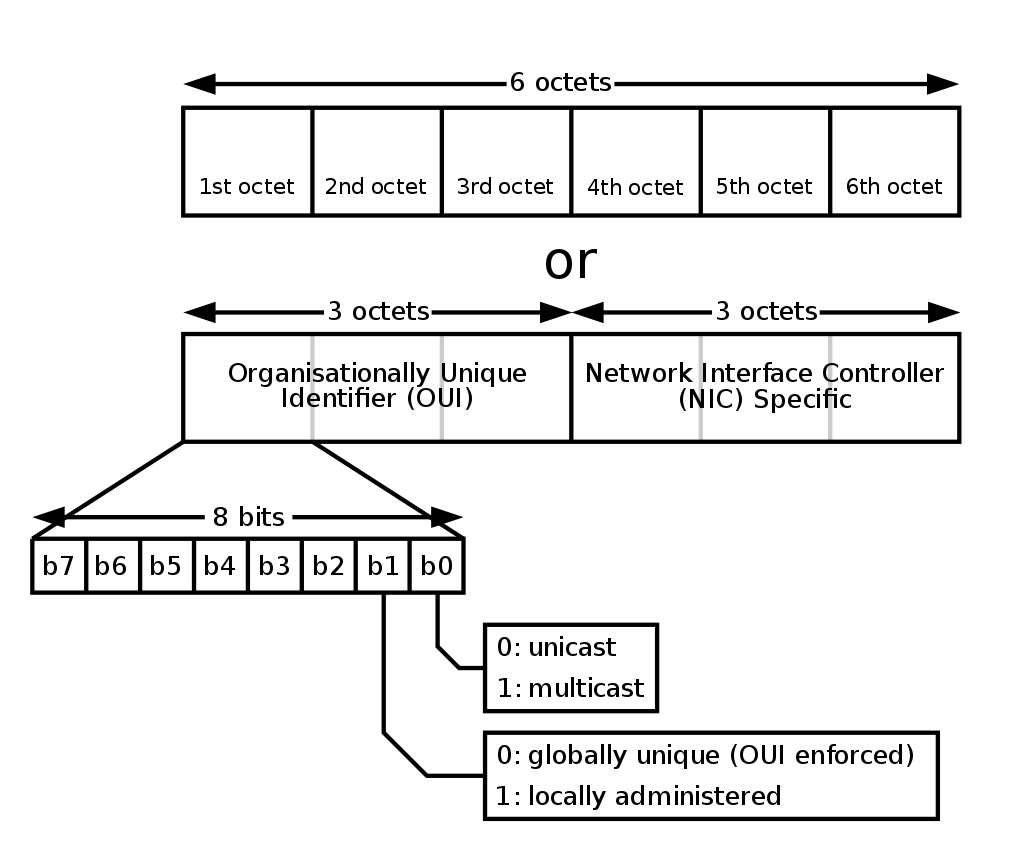
\includegraphics[width=12cm]{images/probe/mac_struc.png}
	\caption{Structure de l'adresse MAC}
	\label{fig:macstruct}
\end{figure}

Les 3 octets de poids faible sont variables et change pour chaque carte mère, c'est ce qui rend chaque adresse du même
constructeur unique, il s'agit du \textbf{NIC}.

Les 3 octets de poids fort sont presque fixes pour chaque constructeur, il s'agit du \textbf{OUI}.
Toutefois, les deux bits de poids faible du premier octet peuvent varier (b1 et b0 sur l'illustration).

b0 indique si l'adresse est individuelle, auquel cas le bit sera à 0 (pour une machine unique, unicast) 
ou de groupe (multicast ou broadcast), en passant le bit à 1

b1 indique 0 si l'adresse est universelle (conforme au format de l'IEEE) ou 
locale, 1 pour une adresse administrée localement (ce bit sera crucial concernant l'analyse de la randomisation)

\subsection{Problèmes de vie privée et randomisation}
La propriété d'unicité des adresses MAC soulève évidemment des problématiques liées à la vie privée. 
la vie privée. Par exemple, selon les dires d'Edward Snowden, la NSA se servait des adresses MAC afin de
monitorer les déplacements d'individus.~\cite{hackernews:snowdan}

Le sujet de ce travail de bachelor soulève les même problématiques. Par conséquent, certaines marques
ont mis en place la \textbf{MAC Address randomization}.

\subsection{Randomisation des adresses MAC~\cite{connected:macrandom}}

Depuis 2014, de plus en plus de constructeurs ont mis en place des mesures
afin de protéger la véritable adresse MAC de l'appareil. 

\begin{itemize}
    \item iOS à partir d’iOS 8 ;
    \item Windows depuis Windows 10 ;
    \item Android depuis Android 6.0 (un patch gère également Android 5.0 pour certains appareils) ;
    \item certains drivers Linux depuis le kernel 3.18.
\end{itemize}

L'objectif étant de varier suffisamment régulièrement l'adresse pour que empêcher le traçage. 
Le processus de randomisation n'étant pas strictement standardisé, l'implémentation peut varier pour chaque constructeur. 

Certaines de ces implémentations sont bonnes (iOS randomise les 6 octets de l'adresse MAC2 sauf b1 et b0) alors que d'autres le sont moins (Android possède des OUI fixes pendant la randomisation, ce qui 
permet déjà la divulgation d'informations sur l'appareil.)

\section{Les probes requests}

Les adresses MAC, aléatoires ou non, sont transmises dans chaque trame MAC, ainsi que bien d'autres
informations. Voici leur structure:

\begin{figure}[H]
	\centering
	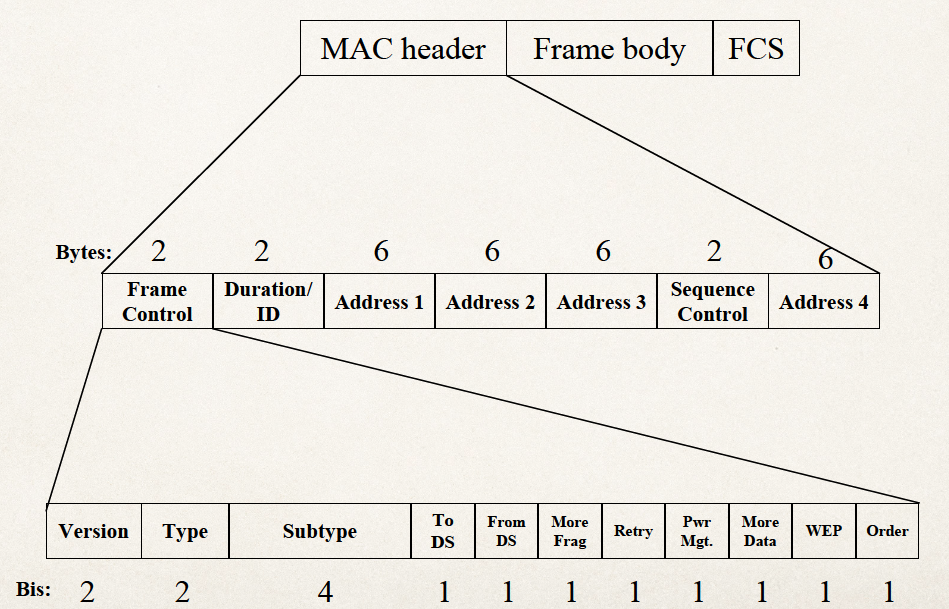
\includegraphics[width=14cm]{images/probe/mac_frame.png}
	\caption{Structure d'une trame MAC}
	\label{fig:macframe}
\end{figure}

On retrouve notamment les adresses MAC de source et de destination dans les champs Address[1|2|3].
Malheureusement, pour qu'un appareil diffuse des trames de \textbf{données}, il faut qu'il soit associé avec un point d'accès. 
Il existe cependant les trames de \textbf{management}. Le champs Subtype (cf figure \ref{fig:macframe}) définit justement
la nature de ces frames. 

Voici les trames de management principales:
\begin{itemize}
    \item Beacon
    \item Probe request \& response
    \item Authentification
    \item Association request \& response
    \item Re-association request \& response
    \item Disassociation
    \item De-Authentification
\end{itemize}

Les trames \textbf{Beacon} sont utilisées par les point d'accès pour signaler leur existence. 

Les trames d'\textbf{(De-)Authentification} sont utilisées par une station et un point d'accès afin d'établir leur identité (pas de chiffrement à ce stade).

Les trames d'\textbf{(Dis|Re)Association} sont utilisées pour lier un AP et une station après l'authentification.

Les trames de \textbf{Probing} servent à un client (request) à demander à un AP ses informations nécessaires à la connexion (e.g le canal).
L'AP concerné envoie alors une probe response avec les informations. 

Une probe request peut être dirigée (un SSID spécifique est spécifié, on l'appelle alors "directed probe request") ou alors aucun SSID n'est spécifié, dans ce cas
on l'appelle "null probe request"

Pour notre solution de scanning, nous cherchons une trame qui n'a pas d'interaction direct avec un access point préexistant
et qui est envoyée par le client. Parmi les trames de management mentionnées, seul les probe requests respectent ces deux contraintes.

Un autre avantage des probe request est que ces dernières sont envoyées très régulièrement (plusieurs fois par minute)
afin de permettre à l'appareil de trouver rapidement les WiFi disponibles. Elles sont même envoyées en rafale ("burst") afin de couvrir
un maximum de canaux 802.11.

Voici un exemple de Probe request dirigée capturée avec Wireshark :
\begin{figure}[H]
	\centering
	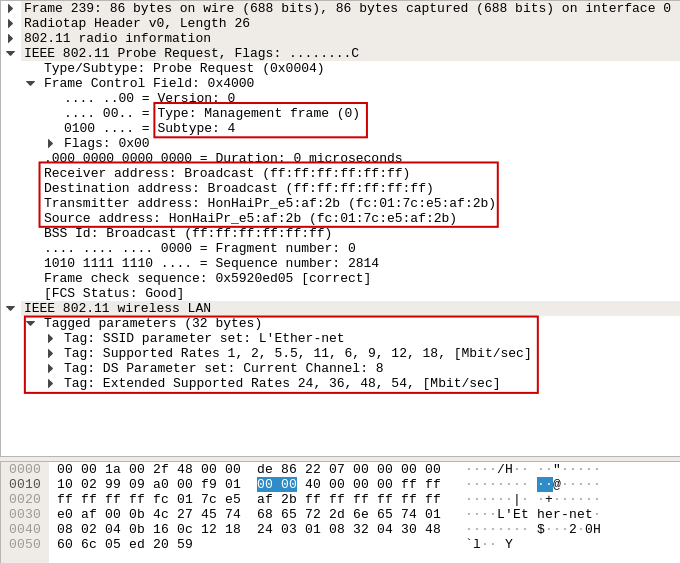
\includegraphics[width=14cm]{images/probe/directed_probe.png}
	\caption{Probe request dirigée}
	\label{fig:directedprobe}
\end{figure}

On y trouve le sous-type de la trame de management qui identifie les Probe requests (4), l'adresse de destination (broadcast)
, l'adresse source (un téléphone Honor 8) et différentes informations dont le \textbf{SSID} recherché : "L'Ether-net"

Les même informations sont disponibles pour une null probe request, mais le SSID est remplacé par un wildcard:
\begin{figure}[H]
	\centering
	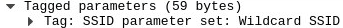
\includegraphics[width=14cm]{images/probe/null_probe_cropped.png}
	\caption{null-probe request}
	\label{fig:directedprobe}
\end{figure}

Il est intéressant de noter que des informations peuvent parfois être déduites des probes requests dirigées.
La plupart du temps, les requêtes sont dirigées car l'appareil s'est déjà connecté au réseau concerné. 
Si le nom du réseau est connu et assez unique, il devient alors possible de déduire où l'appareil se situait par le passé.
Par exemple, sur la figure \ref{fig:directedprobe}, le SSID est l'ancien nom de mon réseau, je peux donc en déduire qu'il s'agit
d'un de mes appareils, et qu'il n'est pas récent. 

Cette technique est aussi utilisée afin de découvrir des réseaux cachés (il s'agit de réseaux qui ne répondent pas aux null probe requests et qui n'envoient pas de beacons).

